\appendix
\section{Architecture}
\label{sec:appA}

\subsection{Common Words Per Year}
In Table \ref{appA:words_per_year} we present a more exhaustive list of the most common words found per year:

\begin{longtable}[H]{>{\raggedright\arraybackslash}p{1cm} >{\raggedright\arraybackslash}p{6cm} >{\raggedright\arraybackslash}p{4cm}}
\caption{Most Common Words by Year} \\
\toprule
\textbf{Year} & \textbf{Common Words} & \textbf{Topic Description} \\
\midrule
\endfirsthead
\toprule
\textbf{Year} & \textbf{Common Words} & \textbf{Topic Description} \\
\midrule
\endhead
\bottomrule
\endfoot
2024 & \textgreek{πανεπιστήμιο, εταιρεία, εκλογή, σχετικά, αγρότης} & University, Elections, Farmers \\
2023 & \textgreek{φωτιά, τετραετία, τουρισμός, περιφέρεια, εκλογή} & Fire, Tourism, Elections \\
2022 & \textgreek{ενεργειακός, ψηφιακός, τουρισμός, πηγή, πόλεμος} & Energy, Digital, Tourism, War \\
2021 & \textgreek{εμβολιασμός, ψηφιακός, εμβολιάζω, υφυπουργός, γραμματέας} & Vaccines, Digital Campaigns \\
2020 & \textgreek{τουρισμός, νησί, νοσοκομείο, ψηφιακός, κορονοϊός} & Tourism, COVID-19 \\
2019 & \textgreek{βουλευτής, εκλογή, ψηφίζω, πλειοψηφία, κόμμα} & Elections \\
2018 & \textgreek{αναπτυξιακός, μνημόνιο, περιφέρεια, παραγωγικός, δημοσιονομικός} & Development, Memorandum \\
2017 & \textgreek{παραγωγικός, περιφέρεια, αναπτυξιακός, παραγωγή, σχεδιασμός} & Production, Regional Development \\
2016 & \textgreek{νησί, διαπραγμάτευση, δικαιοσύνη, κόμμα, αξιολόγηση} & Island Politics, Justice \\
2015 & \textgreek{κυπραίικος, βέβαιος, διαπραγμάτευση, βουλευτής, τράπεζα} & Cyprus Issue, Banking \\
2014 & \textgreek{ευρώ, οικονομικό, κρίση, σχέδιο, ανάκτηση} & Economic Crisis, Recovery Plan \\
2013 & \textgreek{πλεόνασμα, κόμμα, ανταγωνιστικότητα, πρωτογενής, ανεργία} & Surplus, Competitiveness, Unemployment \\
2012 & \textgreek{ανταγωνιστικότητα, ανταγωνισμός, competitiveness, αποκαθιστώ, διατηρώ} & Competitiveness, Market Dynamics \\
\bottomrule
\label{appA:words_per_year}
\end{longtable}

\section{Experimental Setup}
\label{sec:appB}
\subsection{Evaluation Metrics}
\begin{figure}[H]
\centering
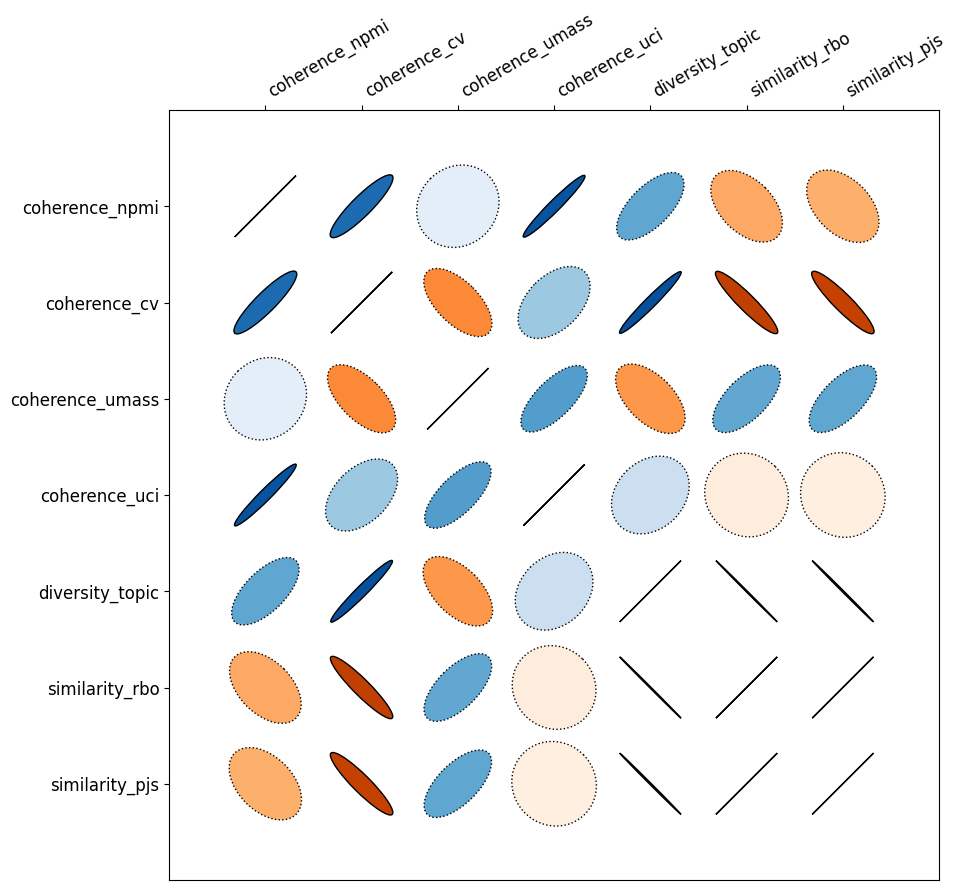
\includegraphics[width=1\columnwidth]{figs/metric_correlations.png}
\caption[Topic Modeling Metric Correlation Matrix]{Metric Correlation Matrix}
\label{appB:metric_correlations}
\end{figure}

\subsection{Hyperparameters}

Below we present the lists of hyperparameters for the NMF model:

\begin{table}[H]
\centering
\begin{tabular}{@{}lc@{}}
\toprule
Parameter           & Value   \\
\midrule
kappa               & 1.0     \\
minimum\_probability& 0.0543  \\
\bottomrule
\end{tabular}
\caption{NMF Hyperparameters}
\end{table}

\subsection{Sentence Transformers}
Document-level granularity models performed significantly better when it comes to the metrics, something we expected because of the constrained amount of topics. Without the topic limitation, sentence-level models produced thousands of topics - with BERTopic's automatic topic reduction not reducing them below four digits. This bottleneck renders their purpose useless and while it would certainly be an interesting topic (pun intended) to explore, it seems out of scope for this analysis.
\begin{table}[h]
    \centering
    \begin{tabular}{@{}lcc@{}}
        \toprule
        Model               & CV Coherence & Topic Diversity \\ 
        \midrule
        gr\_r\_xlm\_sentences       & 0.5019      & 0.9793          \\
        gr\_media\_sentences & \textbf{0.6041}      & \textbf{1.0000}       \\
        multilingual\_sentences & 0.5826  & 0.9724          \\
        gr\_r\_xlm\_docs            & 0.6826    & \textbf{0.7310}          \\
        gr\_media\_docs     &  0.6865    & 0.7241          \\
        multilingual\_docs   & \textbf{0.7024}     & 0.6087          \\
        \bottomrule
    \end{tabular}
    \caption{Model Evaluation on CV Coherence and Topic Diversity}
    \label{appB:st_eval}
\end{table}


\subsection{Topic Representations}
\label{sec:appendix_rep}
As previously mentioned, quantitative metrics aren't reliable measures of the quality of the topics. This becomes more apparent when changing the representation model. The default c-TF-IDF model, as seen in Table \ref{tab:coherence} yields better metrics, but different representations, as seen in Table \ref{tab:topics_compare}, make the topics much more human interpretable.


\begin{table}[h]
\centering
\begin{tabular}{lccc}
\toprule
 & CV Coherence  & UMass Coherence & Topic Diversity \\
\midrule
Default Representation Model & 0.646 & -0.518 & 0.935 \\
Custom Representation Model & 0.335 & -0.592 & 0.957 \\
\bottomrule
\end{tabular}
\caption{Topic Coherence Metrics}
\label{tab:coherence}
\end{table}

\begin{table}[H]
\centering
\begin{tabular}{ll}
\toprule
Default representation & Custom representation \\
\midrule
que, de, en, la, el & \textgreek{δημοκρατία, προνομιακός, μεταρρυθμίσεις} \\
\textgreek{ευρώ, μητσοτάκη, κύριε μητσοτάκη} & \textgreek{σταθερότητα, μνημόνια, κυβέρνηση} \\
\bottomrule
\end{tabular}
\caption{Comparison of Default and Custom Representations}
\label{tab:topics_compare}
\end{table}

\section{Experiments}

\subsection{Best Model Topic Representations}
\label{sec:appExpBest}

\begin{table}[H]
\caption{Top 8 most common topics for the best performing models (in English)}
{\footnotesize 
\begin{tabular}{|c|m{4cm}|m{4cm}|m{4cm}|}
\hline
\textbf{Topic} & \textbf{ProdLDA} & \textbf{BERTopic+} & \textbf{BERTopic} \\
\hline
1 & Obligated, clearance, entrance, minute, overcharge, mouth, enumerate, analyst, objectively & Government, solution, state, reforms, debt, you know, national & \textit{democracy, reforms}, euro, region, development, European, agreement \\
\hline
2 & Energy, presidency, directive, regulation, ultimate, ready, multi-year, adoption, migration, unemployment & Stability, memorandums, government, parliament, reforms, debt, Greek people & Tsipras, elections, Mitsotakis, SYRIZA, euro, Mr. Mitsotakis, ladies gentlemen \\
\hline
3 & Partner, negotiation, regulation, radical, administration, suffocating, institutional, eurozone, claiming, tax & Health system, doctors, nurses, beds, ICU, hospitals, health, Vasilis, vaccination, intensive care & Health, hospital, health system, hospitals, vaccination, national system, system \\
\hline
4 & Freedom, democratic, tolerance, against, racism, order, stereotypes, extremism, enemy, ethos & Prime Minister, Antonis, democracy, privileged, national, interests, simply, EAB, presidency & \textit{que, de, en, la, el}, Samaras, democracies \\
\hline
5 & Clearance, obligated, disastrous, mouth, entrance, writing, stock market, similar, apportion & Minimum wage, primary, new, CAP, minimum, livestock farmers, restaurant industry, businesses & Farmers, agricultural, products, agricultural, primary, sector, products, disability \\
\hline
6 & Hospital, personnel, doctor, care, primary, patient, cancer, governance, nurse, manager & Fires, crisis management, civil protection, EKAB, firefighting, civil protection, citizen, floods & Civil protection, protection, EKAB, civil protection, policy, firefighting, fires, police \\
\hline
7 & City, metro, museum, schedule, kilometer, Olympic, road, station, sports, regeneration & Immigration, asylum, solution, pact, migration, EU, Turkey, identification, flows & Flows, Frontex, refugees, Turkey, border, migration, borders \\
\hline
8 & Needs, add, table of appearances & Western Macedonia, renewable sources, liquefied, ELPE, FSRU, pipeline, ADMIE & Gas, energy, natural gas, natural gas, natural gas, natural \\
\hline
\end{tabular}}
\begin{tablenotes}
\small
\item \textit{Words in italics were found in the same language as presented here}
\end{tablenotes}
\label{appTab:english_topics}
\end{table}